\pagestyle{fancy}
%%%%% Physical motivation
%%%%% Standard model
\section{Standard Model} \thispagestyle{fancy}

The Standard Model, which was formulated in the 1970s, describes the elementary particles and the interactions between them.
It combines the theory of the elementary particles, quantum mechanics, quantum chromodynamics (strong interactions), and electroweak forces (unified description of the weak and electromagnetic forces). 
While most of its assumptions were confirmed in the 1980s, the most recent one - the confirmation of the existence of the \emph{Higgs boson}, dates from 2013. \cite{zbroszczyk}

However, the Standard Model is not complete, as it does not describe e.g., the gravitational force, or the new findings such as the existence of the dark matter and the muon's magnetism \cite{standard model}. While the explanation of these phenomena could prove the theory wrong, it describes well the majority of interactions between matter.

According to the Standard model, there are two main classes of elementary particles: \textbf{fermions}, which constitute matter, and  \textbf{bosons}, which carry interactions. They are presented on Figure \ref{standard} and described below.

\begin{figure}[H]
    \centering
    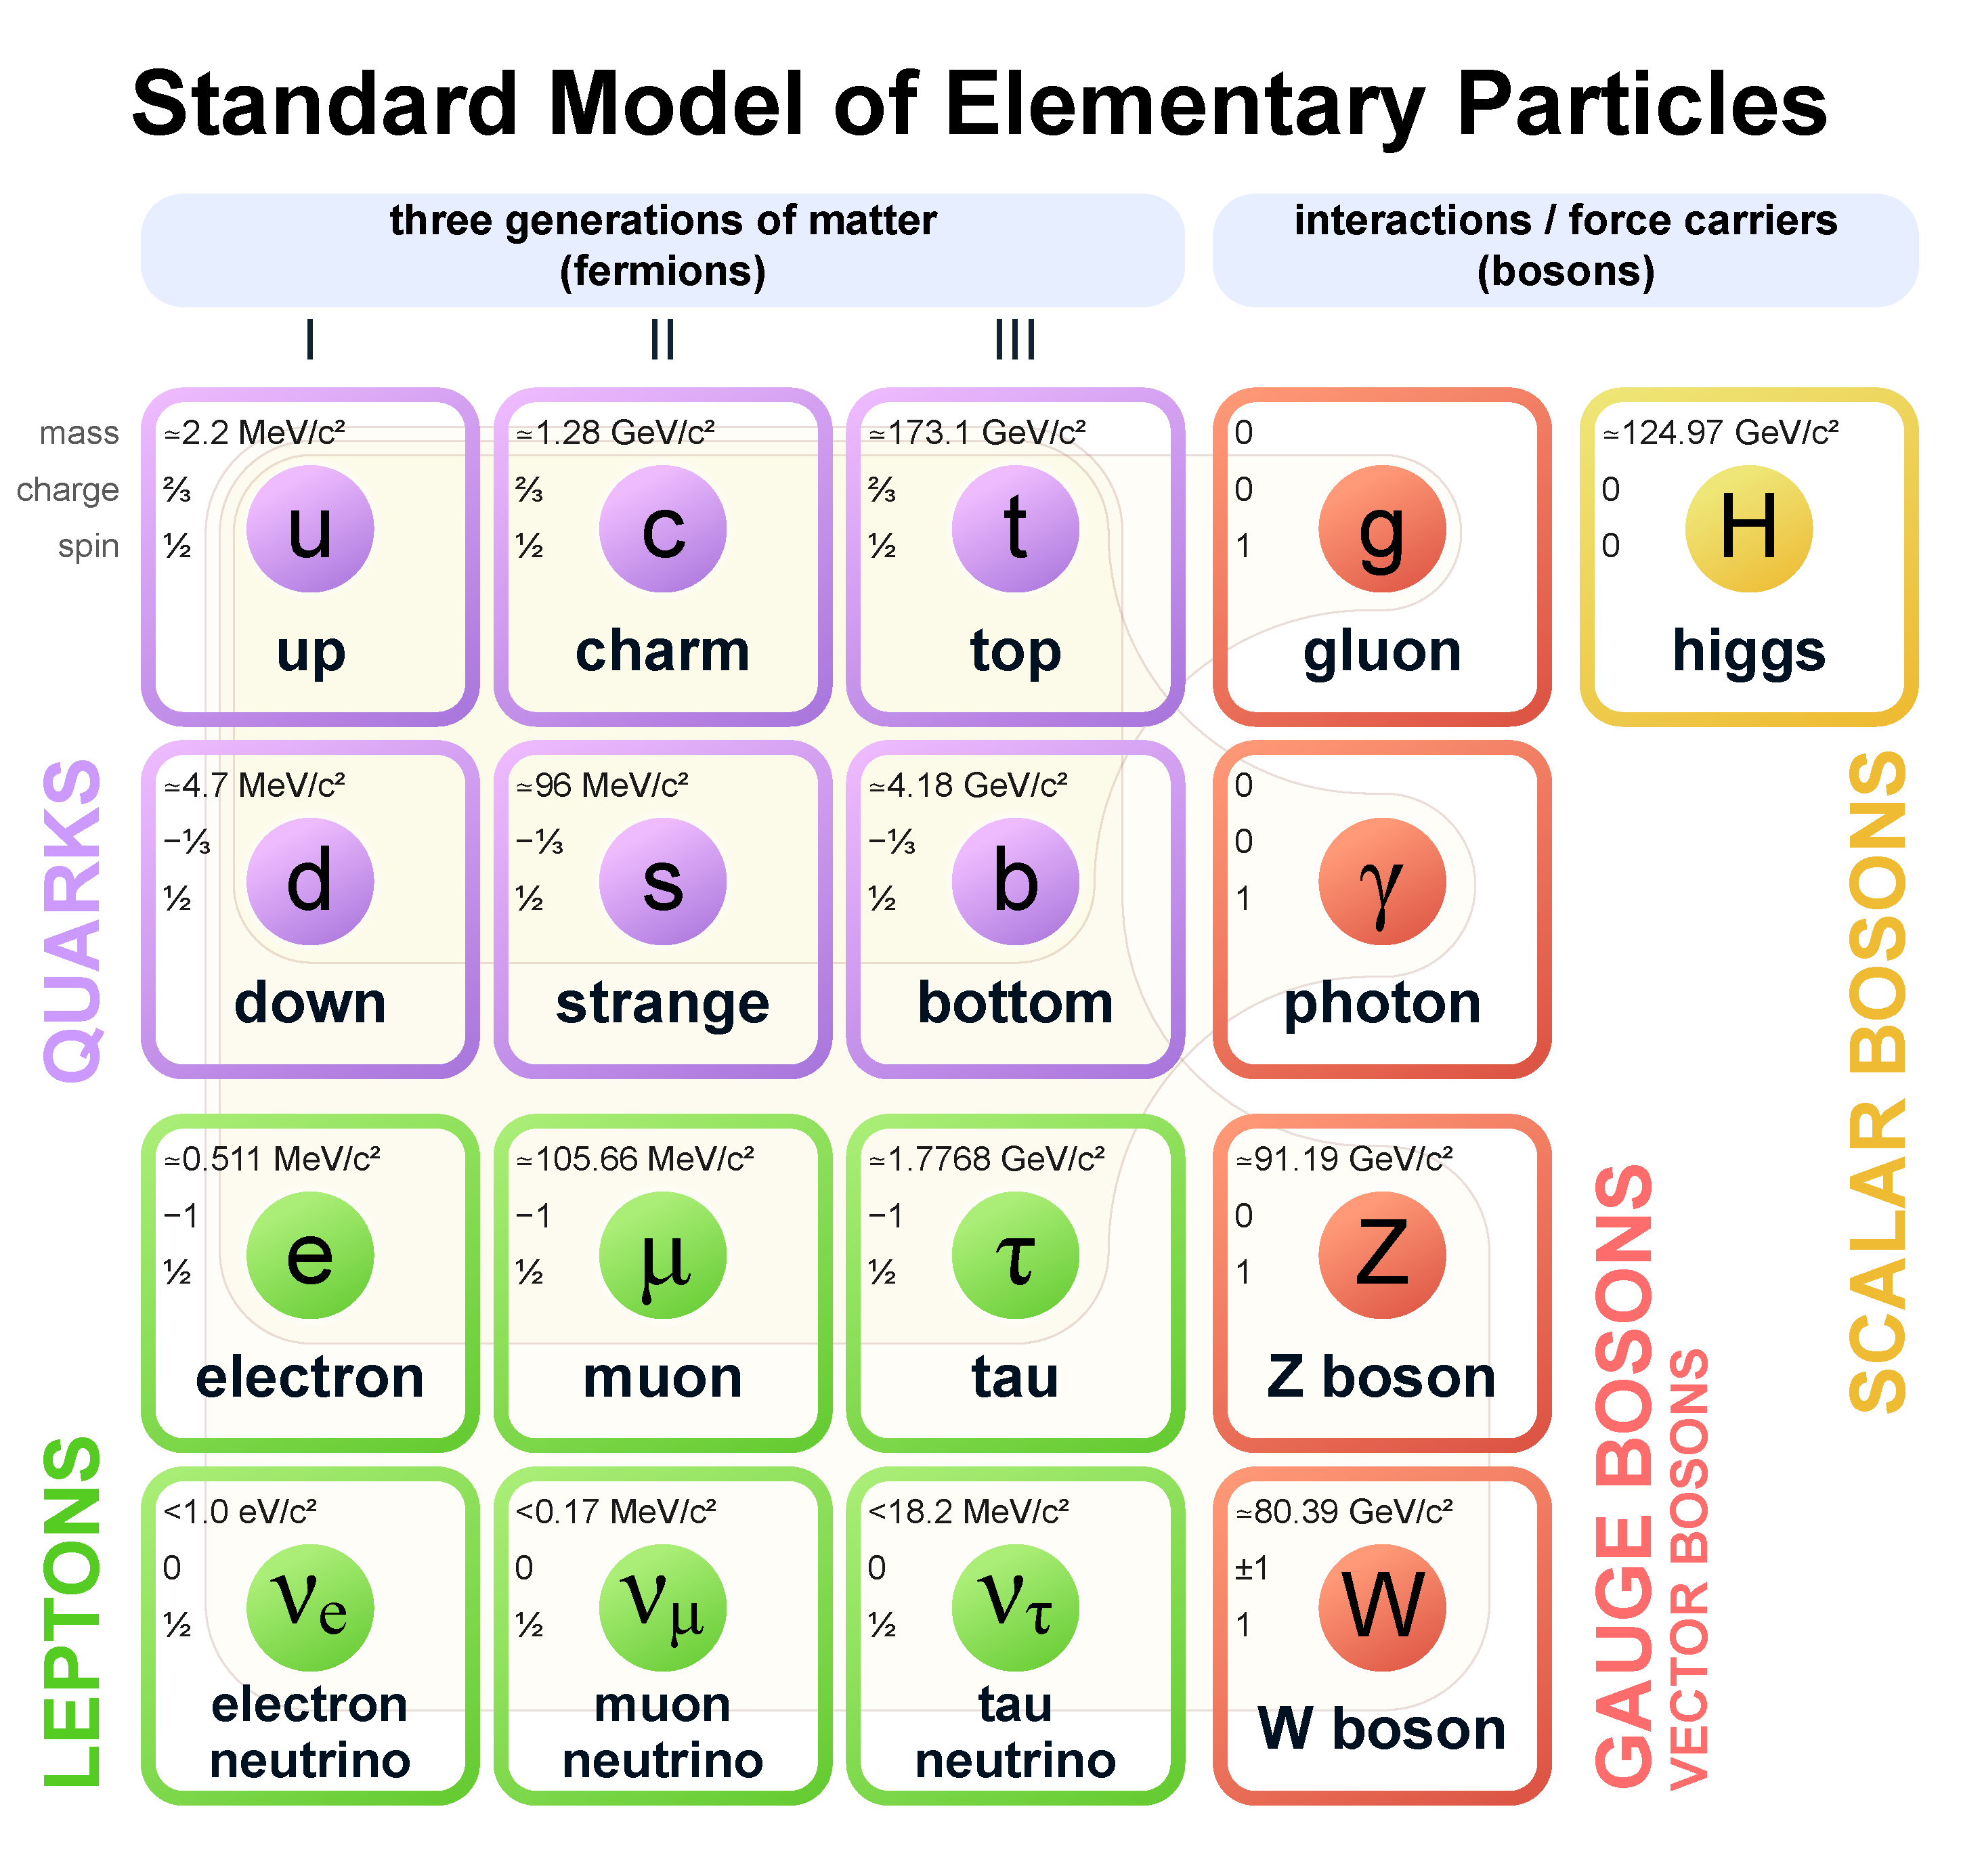
\includegraphics[width=.58\textwidth]{inz_szablon_new/img/Standard Model of Elementary Particles.pdf}
    \caption{Standard Model of Elementary Particles \cite{wiki}}
    \label{standard}
 \end{figure}

Fermions follow the Fermi-Dirac statistics (hence the name), they have half odd integer spin and thus follow the \textbf{Pauli exclusion principle}. They can be divided into two groups: \textbf{leptons} and \textbf{quarks}. Leptons, unlike the quarks, have an integer charge number; they do not have the \textbf{color charge}, so they do not engage in strong interactions. There are three generations of fermions: 
\begin{enumerate}[label=\Roman*.]
    \item quarks: \emph{up (u)} and \emph{down (d)}; leptons: \emph{electron} (\Pem) and \emph{electron neutrino} (\Pgne)
    \item quarks: \emph{charm (c) and \emph{strange (s)} }; leptons: \emph{muon} (\Pgmm) and \emph{muon neutrino} (\Pgngm) 
    \item quarks: \emph{top (t)} and \emph{bottom (b)}; leptons: \emph{tau} (\Pgtm) and \emph{tau neutrino} (\Pgngt)
\end{enumerate}

   
Bosons follow (\emph{nomen omen}) Bose-Einstein statistics, they have an integer spin. There are five elementary bosons carrying: 
\begin{itemize}
    \item strong forces: \emph{gluons} (\Pg)
    \item weak forces: bosons \PWpm and \PZz
    \item electromagnetic forces: \emph{photons} (\Pgg)
    \item mass: \emph{Higgs boson} (\PH) 
\end{itemize}

%%%%% Standard model
\section{Quantum chromodynamics}
Quantum chromodynamics, a part of the Standard Model theory, describes strong interactions between quarks and gluons. It explains i.a. why quarks are confined in the hadrons\cite{zbroszczyk}. According to this theory:
\begin{itemize}
    \item there are three color charges: \emph{Red}, \emph{Green}, and \emph{Blue} which are exchanged between the quarks via bosons - \emph{gluons}
    \item gluons interact with both quarks and other gluons
    \item the strong interaction has a pulling character, the \emph{color potential} can be described by this formula:
\end{itemize}
\begin{equation} \label{qcd potential}
    V (r) = - \frac{4}{3} \frac{\alpha_s}{r} + kr 
\end{equation}
where $\alpha_s$ and $k$ - coupling constants, $r$ - distance.
According to the formula \ref{qcd potential}, the magnitude of the force grows with distance, unless the latter is bigger than a certain threshold (as shown on Figure \ref{qcd graph}) - then, a new particle-antiparticle couple is created. This effect, called \textbf{quark confinement}, explains why the quarks cannot be separated and form \textbf{hadronic matter}. However, if the distance $r$ is very small, and the energy of the system is big enough, there exists another state of matter called \textbf{quark-gluon plasma (QGP)} for which the quarks reach asymptotic freedom (asymptotic, as the strong interactions still do not allow the existence of \emph{free} quarks).
\begin{figure}[H]
    \centering
    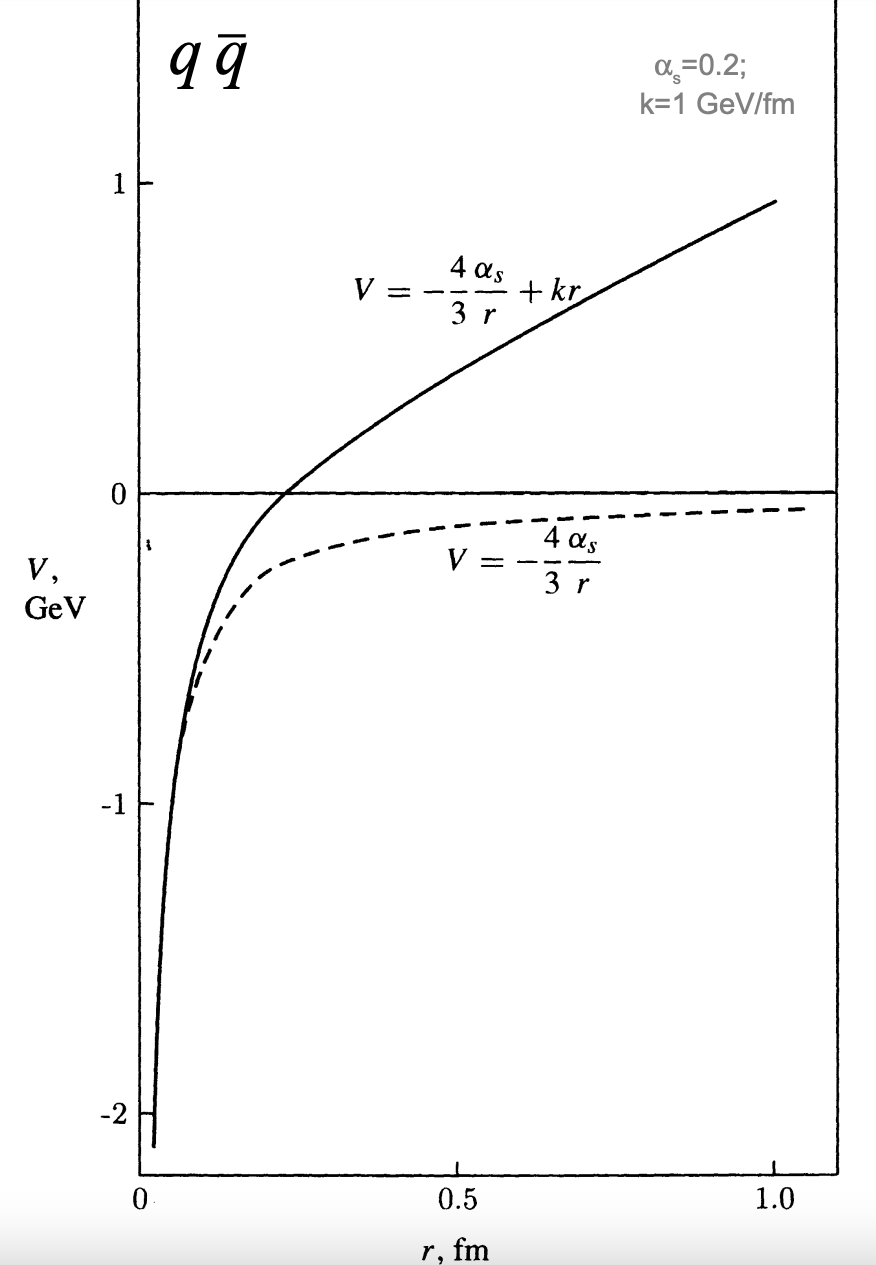
\includegraphics[width=.5\textwidth]{inz_szablon_new/img/qcd potential.png}
    \caption{Dependence of the color charge potential and the distance between the quarks and gluons. At long distances, the binding energy is too high and a new particle-antiparticle pair is created \cite{grebieszkow}}
    \label{qcd graph}
 \end{figure}
 As the matter can exist in both states: \emph{hadronic matter} and \emph{QGP}, the phase transition between the two is certain. The phase diagram can be presented on a 2D graph (with net baryon density on the \emph{x}-axis and temperature on the \emph{y}-axis) (Figure \ref{phase 2d}). The QCD matter diagram, especially the phase transition, is investigated by multiple high-energy physics experiments.
 \begin{figure}[H]
 \centering
    \centering
    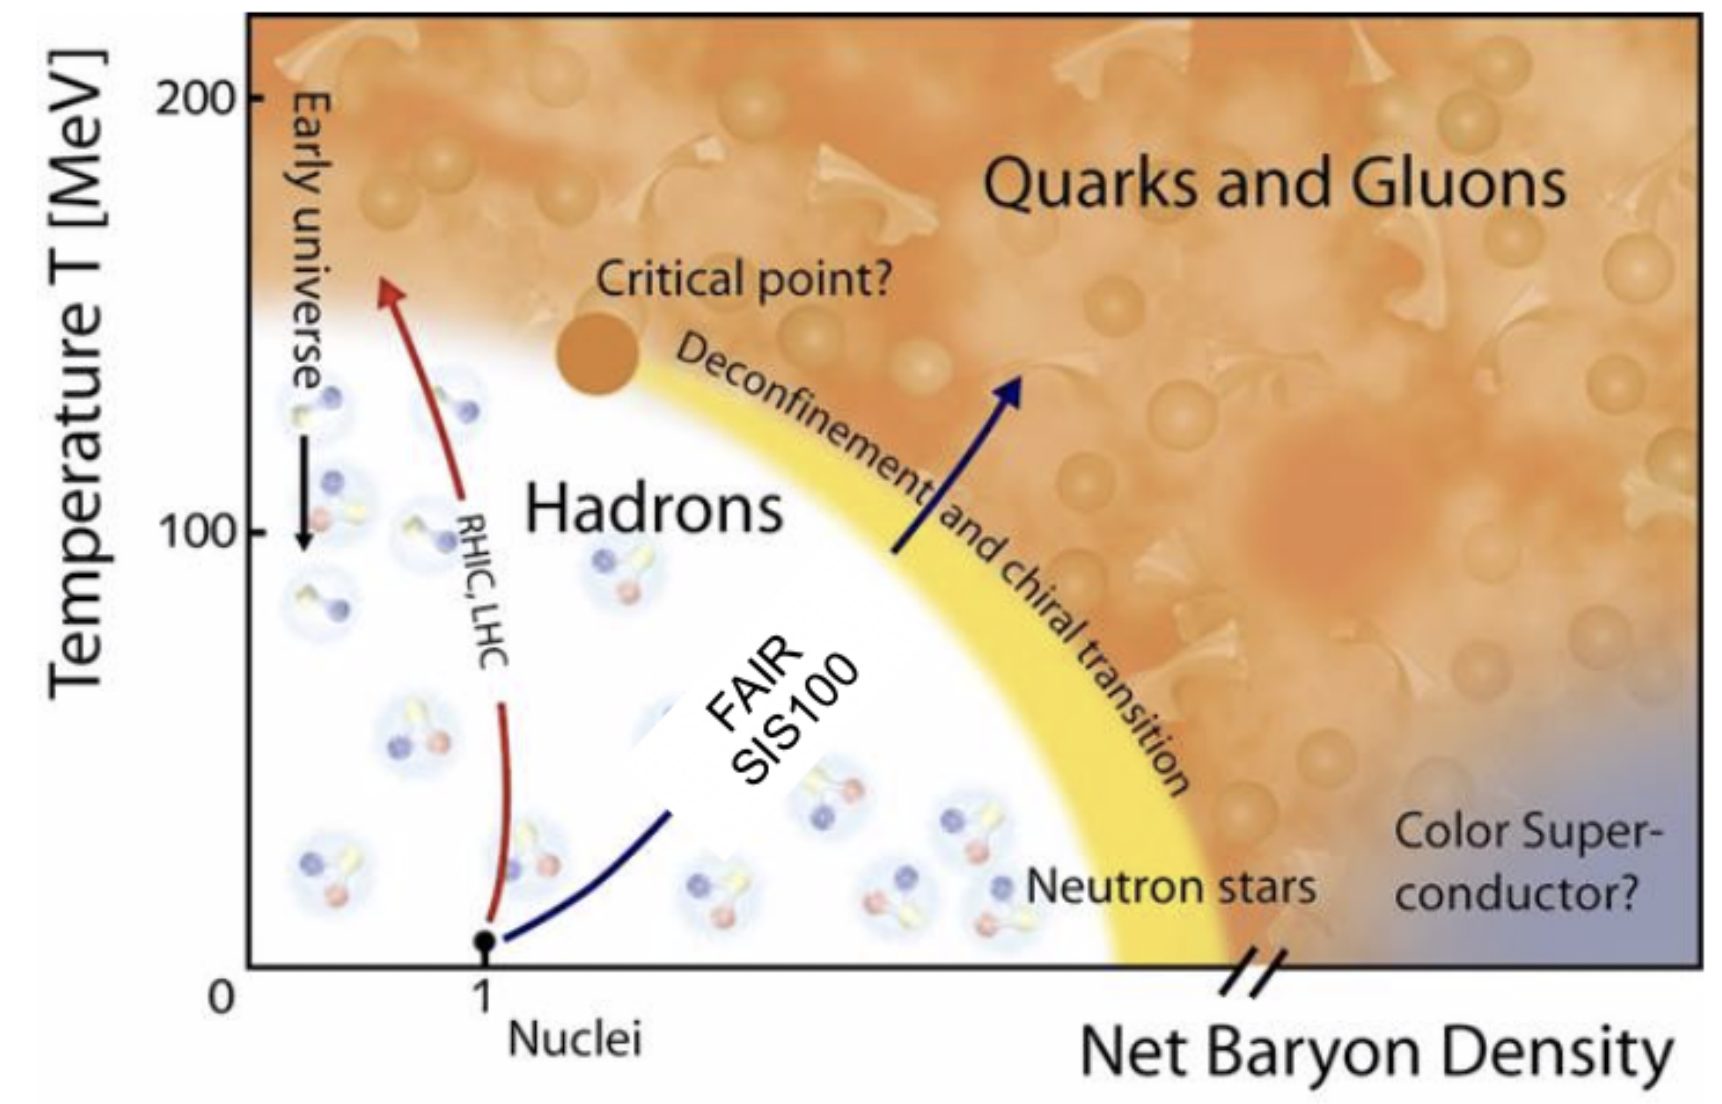
\includegraphics[width=.7\textwidth]{inz_szablon_new/img/phase_diagram2d.png}
    \caption{Phase diagram of the QCD matter  \cite{progress report}}
    \label{phase 2d}
    \vspace{0.3cm}
\end{figure}
%%%%%%%%%%%%% Heavy-ion collisions
\section{Heavy-ion collisions}
Heavy-ion collisions at relativistic energies allow achieving both high temperature and high net baryon density, consequently  creating \emph{QGP} for a short time. In the \emph{fixed-target} experiments, a heavy-ion is aimed at e.g., a foil; in the \emph{collider} experiments, two heavy-ions are accelerated and then collided, allowing to achieve higher energies.

\begin{figure}[H]
    \centering
    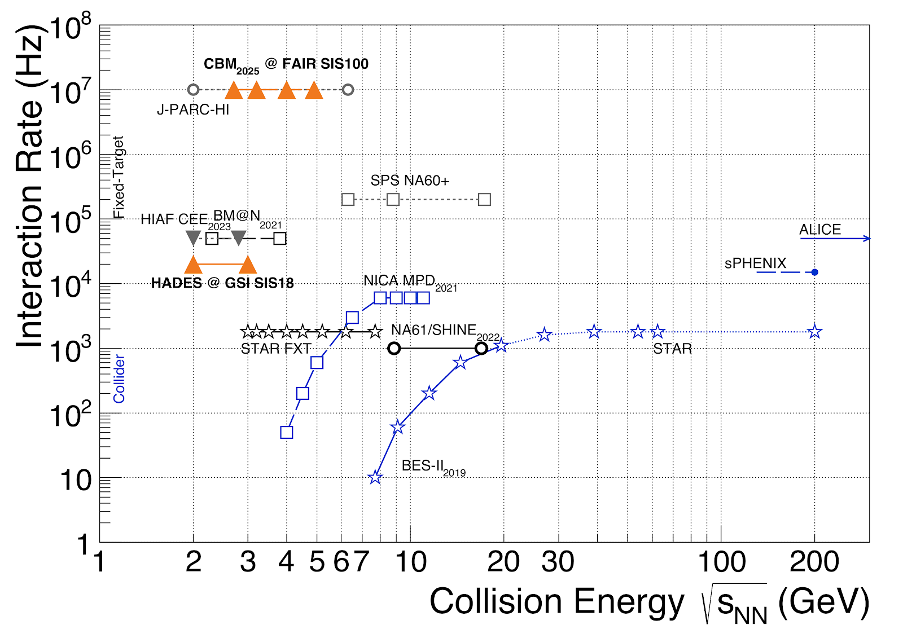
\includegraphics[width=.8\textwidth]{inz_szablon_new/img/hep map.png}
    \caption{The "map" of the heavy-ion collision experiments \cite{hep map}}
    \label{hep experiments}
 \end{figure}

Besides the type of setup, the high energy physics experiments also differ from one to another by i.e. achieved temperature, interaction rate, atomic number of the \emph{bullet} (collided) ion, etc. The most important, current experiments are shown on the Figure \ref{hep experiments}. As we see on both Figure \ref{phase 2d}, and Figure \ref{hep experiments}, while the experiments at the Large Hadron Collider (LHC) in CERN aim for bigger collision energies and hence temperatures\cite{alice}, the experiments performed (or planned) on SIS accelerators in FAIR aim for bigger interaction rates and consequently bigger net baryon density\cite{sis}.

%%%%%%%%%%%%% Strange particles
\section{Reconstruction of short-lived strange particles}
In the heavy-ion experiments, the strange quarks are only produced during collisions. Thus, they provide information about the evolution of nuclear matter. It is expected\cite{deconfinement} that in the \textbf{mixed-phase} (when both nucleon and quark degrees of freedom are present), which can be produced at FAIR energies, the yield of strange particles could be comparable with particles composed of \emph{u} and \emph{d} quarks (as shown on Figure \ref{mixed}). To verify this, the reconstruction of strange particles, also short-lived ones  like \textit{$\Lambda^0$}, \textit{$\Xi^-$}, \PKzS which cannot be detected directly, is important.

\begin{figure}[H]
    \centering
    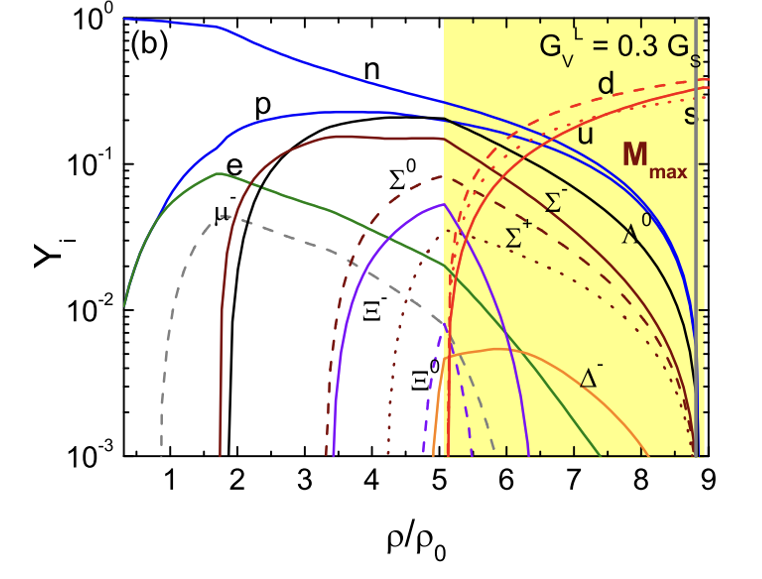
\includegraphics[width=.6\textwidth]{img/mixed_phase.png}
    \caption{Particle population vs density (mixed-phase highlighted in yellow) \cite{deconfinement}}
    \label{mixed}
\end{figure}